\documentclass[10pt,a4paper]{article}
\usepackage[T1]{fontenc}
\usepackage[utf8]{inputenc}
\usepackage{newtxtext,newtxmath}
\usepackage[a4paper,textwidth=150mm,textheight=235mm,centering,headheight=13pt]{geometry}
\usepackage{microtype,amsmath,booktabs,tabularx,array,longtable,graphicx}
\usepackage[numbers,sort&compress]{natbib}
\usepackage[french]{babel}
\usepackage{xurl}
\usepackage{fancyvrb,flafter,needspace,placeins}
\usepackage[hidelinks]{hyperref}
\usepackage{fancyhdr,titlesec}
\titleformat{\section}{\large\bfseries}{\thesection.}{.5em}{}
\titleformat{\subsection}{\normalsize\bfseries}{\thesubsection}{.5em}{}
\setlength{\parskip}{4pt}\setlength{\parindent}{0pt}
\setlength{\emergencystretch}{3em}\setlength{\tabcolsep}{4pt}
\renewcommand{\arraystretch}{1.15}\renewcommand{\bibfont}{\footnotesize}
\renewcommand{\thesection}{S\arabic{section}}
\setcounter{secnumdepth}{2}
\pagestyle{fancy}\fancyhf{}\fancyhead[L]{\small HealthGraphBench | RC2}
\fancyhead[R]{\small Supplément scientifique}\fancyfoot[C]{\small\thepage}
\renewcommand{\headrulewidth}{0pt}\raggedbottom
\clubpenalty=10000\widowpenalty=10000
\newcommand{\src}[1]{{\small\nolinkurl{#1}}}
\hypersetup{pdftitle={HealthGraphBench RC2 — Supplément scientifique},pdfauthor={},pdfsubject={Version de travail RC2; validation des auteurs requise}}
\begin{document}

\begin{center}
{\small SUPPLÉMENT SCIENTIFIQUE • VERSION DE TRAVAIL RC2 — non approuvée par les auteurs}\par\vspace{7pt}
{\LARGE\bfseries HealthGraphBench — RC2}\par\vspace{6pt}
{\large Méthodes, traçabilité et analyses complémentaires}
\end{center}

\textbf{Organisation actuelle.} Le supplément commence par les définitions et configurations des méthodes (S1), puis la carte des preuves (S2). Les populations sont en S3 et la chronologie scientifique courte en S4. Les résultats et contrôles historiques S5--S10 restent séparés de l'exploration MAUDE de durée, du rapprochement apparié et du diagnostic secondaire D1 en S11. Le registre détaillé des versions et leurs statuts est conservé dans la provenance, non présenté comme une suite de nouvelles expériences.

\par\Needspace{8\baselineskip}
\section{Définitions et configurations des méthodes}
\label{supp:methods}
\subsection{MAUDE : historiques, heuristiques et entraînement}
Pour un produit $p$, $H_p$ est l'ensemble des problèmes antérieurs et $U_c$ l'ensemble des produits historiquement associés au problème $c$. L'ensemble des pairs est $N_p=(\bigcup_{d\in H_p}U_d)\setminus\{p\}$. La fréquence des voisins vaut $|N_p\cap U_c|$ ; la popularité globale vaut $|U_c|$. Chaque produit pair contribue une fois, indépendamment de son volume de signalements ou du nombre de problèmes partagés. Il n'existe ni pondération de Jaccard ni normalisation par degré dans cette heuristique MAUDE. L'absence de soutien donne zéro. Les candidats sont tous les problèmes antérieurement connus hors $H_p$ ; les égalités suivent score décroissant, soutien global décroissant, puis code croissant\cite{hgbcode}.

Les douze variables tabulaires sont : logarithmes $\log(1+x)$ des signalements antérieurs du produit et du problème, du nombre de produits associés au problème, du nombre de voisins qui lui sont associés et du nombre de produits associés pendant les quatre derniers trimestres ; fraction récente du soutien du problème ; logarithmes du nombre de fabricants du produit et de l'activité cumulée de leurs produits ; âges du produit et du problème en trimestres ; logarithme de la prévalence du problème parent ; fraction récente des signalements du produit. Elles incluent donc déjà de l'information relationnelle : « tabulaire » ne signifie pas « strictement local ».

Le chemin tabulaire accumule les premiers liens admissibles et un non-positif historique déterministe par positif, avec caractéristiques construites avant l'ajout du trimestre cible. Les réajustements de 2023T1, 2024T1 et 2025T1 utilisent uniquement les lignes déjà accumulées. Les méthodes fondées sur les embeddings ajustent leur représentation sur le graphe historique disponible à ces réajustements, et non sur un même tableau de premières apparitions. Cette différence d'objectif et d'exemples interdit d'attribuer leur écart à la seule agrégation.

\begin{tabularx}{\linewidth}{@{}p{36mm}X@{}}
\toprule
Méthode & Constantes du chemin gelé et qualification\\
\midrule
Logistique MAUDE & 40 époques ; taux d'apprentissage 0,15 ; $L_2=0,01$ ; standardisation sur les lignes d'entraînement.\\
Arbres boostés & Arbres à un niveau ; 12 tours ; taux d'apprentissage 0,08.\\
Factorisation spectrale & Rang 8 ; 18 itérations.\\
BPR + moyenne fixe à un saut & Dimension 8 ; 4 époques ; combinaison après apprentissage : 0,5 vecteur de la cible et 0,5 moyenne des vecteurs voisins. Il n'y a pas de propagation apprise de bout en bout.\\
GraphSAGE à un saut & Dimension 8 ; 3 époques ; 8 voisins ; taux d'apprentissage 0,02 ; régularisation 0,0005 ; perte BPR ; activation $\tanh$ ; vecteurs de nœuds entraînables et transformations partagées.\\
Exploration de durée C & Même configuration GraphSAGE ; fits indépendants 0/3/10/30 sur validation, puis 30 sélectionné. Rapprochement apparié avec les voisins conservés et IC conditionnel par produit en S11.\\
Diagnostic secondaire D1 & Mean30 conservé de C ; none30 self-only non-GNN, appris par BPR sur les mêmes arêtes. Durée imposée depuis mean, perte presque plate ; pas d'effet causal isolé.\\
\bottomrule
\end{tabularx}

GraphSAGE échantillonne des voisins ; les exemples négatifs sont déterminés par des hachages, sans générateur aléatoire à l'exécution selon les métadonnées du dépôt. Cela garantit la reproductibilité de cette exécution, pas la stabilité des résultats si les choix changent.

Aucune capacité de généralisation inductive aux nœuds absents du dernier réajustement n'est évaluée séparément. Ces cas reçoivent le score de repli zéro; leur fréquence dans les observations évaluées est documentée en S10. Les triplets BPR dépendent du graphe historique au réajustement. Employer la même fonction de perte ne rend pas ces exemples comparables aux lignes tabulaires.

Les effectifs tabulaires des trois réajustements historiques, les inventaires de graphes et les nombres de triplets/pas impliqués par les boucles sont reconstruits à partir des archives et historiques préparés ; le détail est en S10. Ces reconstructions B1/B2 ne lisaient pas les checkpoints historiques et leurs nombres de pas sont des implications du code gelé, non des journaux d'optimiseur observés. En revanche, les nouveaux checkpoints bruts C/D1 ont été inspectés et audités numériquement comme décrit en S11. L'exploration D1 fournit une comparaison mean/none, mais pas un effet isolé à capacité égale. Le diagnostic synthétique distinct du noyau extrait reste décrit en S8\cite{hgbcode,hgbresults,hamilton2017}.

\subsection{CMS : deux logistiques, et non un duel GNN--tabulaire}
Les modèles emploient onze caractéristiques numériques locales et des indicatrices d'État : comptes antérieurs d'inspections et de déficiences sérieuses, taux antérieur, comptes d'inspections et de déficiences dans des fenêtres de 365 et 730 jours, délai depuis l'inspection précédente, âge de l'établissement et comptes de changements de propriétaire antérieurs et sur 365 jours. Les comptes sont transformés par $\log(1+x)$ ; le délai est plafonné à 1\,460 jours puis divisé par 365,25 ; l'âge est plafonné à 100 ans. Les taux ne sont pas logarithmés.

L'augmentation ajoute douze variables : comptes de propriétaires, de pairs et de pairs avec historique ; inspections et déficiences antérieures des pairs et leur taux ; inspections et déficiences des pairs sur 365 jours et leur taux ; déficiences des pairs sur 730 jours ; nombres de pairs avec au moins une déficience sur 365 et 730 jours. Les comptes sont logarithmés. Les taux sont des rapports de totaux, avec zéro pour dénominateur nul ; ce n'est pas une moyenne non pondérée des taux d'établissements.

Les identifiants CHOW \src{PAC:associate} sont prioritaires. Pour les CCN sans enregistrement dans cette représentation, le code utilise les noms courants normalisés, avec filtres de rôles. Ce choix est un repli, non une union systématique. Les CCN pairs sont dédupliqués et la cible est exclue. Une date de début antérieure ou égale à la cible suffit au filtre ; les dates de fin incomplètes empêchent d'assimiler ce filtre à une histoire juridique complète. Les noms ne certifient pas l'identité d'une personne morale. Les inspections des pairs restent strictement antérieures à la cible. Ces limites concernent la disponibilité historique aussi bien que la résolution des entités\cite{hgbcode}.

Les deux logistiques sont standardisées sur les données d'entraînement et ajustées avec 300 itérations, un taux d'apprentissage de 0,08 et $L_2=0,05$. Pour l'année $y$, les lignes 2019 à $y-1$ sont utilisées. La référence de prévalence est la proportion de positifs dans cet entraînement ; elle est constante pendant l'année cible, puis recalculée l'année suivante. Le score est reconstruit juste avant l'inspection Health Standard ; le modèle ne prédit pas le calendrier des inspections.

\subsection{Part D : représentations et références}
Les lignes sont projetées sur le nom générique exact après retrait des espaces périphériques. Les noms génériques vides sont exclus ; les volumes et spécialités sont agrégés au niveau prescripteur--générique--année. Cela ne réalise ni correspondance RxNorm ni équivalence clinique. Le score de spécialité compte les prescripteurs ayant le médicament dans leur historique et la même spécialité dans leur dernière année observée. Une spécialité absente ou non unique déclenche un repli sur la popularité globale.

Le recouvrement somme les similarités de Jaccard entre l'historique de la cible et ceux de ses pairs ayant au moins un médicament commun, pour les pairs historiquement associés au candidat. Ni le volume de prescriptions ni le nombre total de pairs ne normalise cette somme. Les égalités suivent score décroissant, soutien global antérieur décroissant et clé générique croissante\cite{hgbcode,hgbpartd}.

La logistique utilise dix variables : soutien global en prescripteurs, volume global et volume moyen, taille et volume de l'historique du prescripteur, nombre d'années d'histoire du médicament et variable d'âge, soutien par spécialité, fraction par spécialité et présence de la spécialité. Les variables de compte/âge désignées \src{log_*} sont transformées dans le chemin source. L'entraînement considère des relations historiques positives, avec jusqu'à cinq non-relations historiques par positif ; les négatifs servent à l'entraînement seulement.

La logistique utilise 18 époques, un taux d'apprentissage de 0,10 et $L_2=0,01$. BPR utilise une dimension de 12, cinq époques, trois négatifs par positif, un taux d'apprentissage de 0,03, une régularisation de 0,001 et un poids de spécialité de 0,35 ; aucune propagation de messages n'y est exécutée. Les modèles sont réajustés avant chaque cible 2023/2024. Aucune recherche exhaustive ni égalisation des budgets n'est attestée.

\par\Needspace{17\baselineskip}
\subsection{Contrôle synthétique : ce qui est effectivement mesuré}
\label{supp:control}
Le contrôle \src{healthgraphbench/controls/synthetic.py}, relu au commit épinglé, projette les associations dont la date de début précède le 1\textsuperscript{er} janvier 2024 en voisinages de CCN. Ce filtre ne certifie pas une histoire complète de propriété active. Pour chaque nœud, il génère $x_i\sim\mathcal N(0,1)$, calcule la moyenne des $x_j$ voisins, puis la standardise en $z_i$ à partir du sous-ensemble désigné « entraînement » (70\,\% des nœuds). Les étiquettes suivent
\[
Y_i\sim\mathrm{Bernoulli}\!\left(\sigma(-1+0,5x_i+\beta z_i)\right),
\qquad \sigma(a)=(1+e^{-a})^{-1}.
\]
Le code mesure directement l'AUC de $z_i$ et celle de $x_i$ sur les nœuds de test. Le sous-ensemble d'entraînement sert à la standardisation, pas à l'ajustement des logistiques CMS. À $\beta=0$, le signal relationnel n'intervient pas dans les étiquettes, mais le terme local $0,5x_i$ demeure. Les valeurs conservées pour les graines 301, 302 et 303 sont un diagnostic de construction du signal et de mesure; elles ne valident ni les modèles CMS ni GraphSAGE MAUDE\cite{hgbcontrols}. R3 corrige cette interprétation sans réexécuter le contrôle.


\section{Carte des preuves et périmètre de vérification}
\label{supp:evidence}
Le commit \nolinkurl{b010d5a49eae56837a920b2e30dece41c42c0c44} identifie l'état source du benchmark\cite{hgb2026,hgbresults}. Le DOI \nolinkurl{10.5281/zenodo.22796551} désigne v0.2 : sa résolution et le dépôt public Zenodo ont été vérifiés en ligne en R4. Ce DOI ne désigne pas le paquet manuscrit. La complétion ne modifie ni les artefacts expérimentaux gelés ni un dépôt distant.

\begin{tabularx}{\linewidth}{@{}p{31mm}Xp{39mm}@{}}
\toprule
Pièces & Usage dans l'étude & Niveau de vérification\\
\midrule
Définitions des tâches, rapports v0.1/v0.2 et résumé unifié & Cibles, périodes, résultats et intervalles existants & Lecture ciblée documentée en R2; transcriptions conservées en R3\\
Analyse v0.1 & AUC/AP/Brier annuels, effectifs et profondeur d'historique & Valeurs du résumé compact ; P/R au décile extraits séparément en R2 depuis les prédictions gelées\\
Code des trois tâches & Heuristiques, conventions, constantes d'entraînement, égalités & Lecture ciblée R2, non audit exhaustif; description conservée\\
Historique et mémo ClinicalTrials & Sélection des tâches et motifs de report & Traces disponibles, pas journal complet des décisions humaines\\
Fichiers individuels MAUDE, classements Part D et prédictions CMS & Entrées des analyses complémentaires & Empreintes revérifiées, téléchargements réseau et trois rejeux réels exécutés en R4\\
Résultats C/D1 post-RC1 et checkpoints bruts correspondants & Fichiers de métriques, manifestes, prévols, séries d'époques et audits numériques ; sources C/D1 épinglées & Nouveaux fits vérifiés ; limites d'exposition et de métriques mémoire détaillées en S11\\
Rapprochement GraphSAGE30--voisins & Contributions produit--trimestre alignées, protocole et tirages de l'IC conditionnel & Calcul ciblé du 3 octobre 2026, sans fit ; limites d'appariement et d'incertitude en S11\\
Code du contrôle synthétique & Portée de l\textquotesingle AUC directe & Source relue au commit épinglé pour R3, sans exécution\\
Archives brutes FDA/CMS & Ingestion et reconstruction historique & Neuf archives officielles MAUDE ingérées pour B1/B2; CMS et la reconstruction exhaustive FDA/CMS restent hors portée\\
\bottomrule
\end{tabularx}



\section{Populations et portée des données documentées}
\label{supp:population}
Les tableaux historiques ci-dessous associent les résumés gelés, l'extraction R2 de descripteurs depuis les fichiers individuels et la collecte MAUDE R6 limitée aux archives brutes. Leurs dénominateurs historiques restent inchangés ; les nouveaux dénominateurs C/D1 figurent séparément en S11. Une observation MAUDE est un produit--trimestre avec au moins un lien positif ; une observation CMS est une inspection cible ; une observation Part D est un prescripteur--année admissible. Les unités rééchantillonnées ne remplacent pas ces dénominateurs.

\begin{tabularx}{\linewidth}{@{}p{35mm}rrX@{}}
\toprule
Partition & Observations & Positifs & Précision\\
\midrule
MAUDE validation 2023 & 3\,483 & 7\,705 & Liens positifs ; 1\,641 produits distincts\\
MAUDE test 2024--2025 & 6\,370 & 13\,174 & Liens positifs ; 2\,026 produits distincts\\
CMS validation 2023 & 2\,661 & 408 & 2\,660 CCN distincts\\
CMS test 2024 & 8\,909 & 1\,253 & 8\,881 CCN distincts\\
CMS test 2025 & 10\,076 & 1\,170 & 9\,990 CCN distincts\\
CMS test regroupé & 18\,985 & 2\,423 & 13\,889 CCN distincts\\
Part D validation 2023 & 2\,000 & 5\,794 & Liens ; 1\,035 observations avec positif\\
Part D test 2024 & 2\,000 & 5\,476 & Liens ; 1\,019 observations avec positif\\
\bottomrule
\end{tabularx}
\textbf{Descripteurs Part D récupérés.} Les sorties gelées fournissent aussi les effectifs historiques et d'entraînement, ainsi que la taille des listes de candidats pour les cohortes de validation 2023 et de test 2024. Les quantiles de candidats sont interpolés linéairement sur les 2\,000 prescripteurs admissibles de chaque cohorte.

\begin{table}[!htbp]\centering\small
\caption{Descripteurs de la représentation générique Part D extraits des résultats conservés.}
\begin{tabularx}{\linewidth}{@{}Xrr@{}}
\toprule
Descripteur & Validation 2023 & Test 2024\\
\midrule
Médicaments dans l'historique & 1\,007 & 1\,042\\
Arêtes historiques prescripteur--médicament & 58\,472 & 60\,200\\
Lignes d'entraînement logistique & 337\,702 & 349\,460\\
Dont positives & 58\,472 & 60\,200\\
Dont négatives & 279\,230 & 289\,260\\
Mises à jour des paramètres BPR & 877\,080 & 903\,000\\
Nœuds de spécialité & 71 & 72\\
Replis vers la popularité globale & 0/2\,000 & 0/2\,000\\
Candidats : minimum & 613 & 675\\
Candidats : premier quartile & 974 & 1\,008\\
Candidats : médiane & 997 & 1\,032\\
Candidats : troisième quartile & 1\,004 & 1\,039\\
Candidats : maximum & 1\,006 & 1\,041\\
Moyenne de candidats & 977,764 & 1\,011,9\\
\bottomrule
\end{tabularx}
\end{table}

Ces descripteurs sont transcrits dans \src{data/available_descriptors_R2.json}. L'extraction a vérifié les empreintes SHA-256 des entrées et du rapport source ; elle n'a ni reconstruit les sources brutes ni relancé d'entraînement.

CMS contient 10\,313 observations de test avec une inspection antérieure (1\,341 positives), et 8\,672 avec au moins deux (1\,082 positives). Le rapport caractérise l'historique retenu comme une ou deux inspections. Ces strates ne sont pas un décompte de tous les soins ou inspections jamais reçus par les établissements. Les extraits courants, leur sélection de fournisseurs et leur nombre limité de cycles tronquent l'histoire\cite{hgbanalysis,hgbresults}.

\textbf{Entraînement CMS reconstitué.} Soient $n_0,p_0$ les effectifs avant 2023, et $c_{23},c_{24}$ les constantes de prévalence enregistrées : 0,1181026137463698 et 0,13793103448275862. Le protocole annuel ajoute les 2\,661 inspections de 2023 et leurs 408 positifs\cite{hgbcode}. Sous ce protocole,
\[
 c_{23}=p_0/n_0,\quad c_{24}=(p_0+408)/(n_0+2661),\qquad
 n_0=\frac{408-2661c_{24}}{c_{24}-c_{23}}=2066.
\]
On obtient $p_0=244$, puis les effectifs ci-dessous. La constante 2025 est retrouvée indépendamment comme $1905/13636=0,1397037254326782$. Les entiers et les trois rapports sont contrôlés numériquement par \src{summary_identities_R4.py}.
\begin{table}[!htbp]\centering\small
\caption{Effectifs CMS reconstruits algébriquement sous le protocole déclaré, non lus directement dans les lignes d'entraînement.}
\input{tables/cms_training_R4_fr.tex}
\end{table}

\par\Needspace{5\baselineskip}
\textbf{Descripteurs MAUDE extraits.} L'exécution de \src{extract_descriptors_R4.py} sur le fichier gelé vérifié donne, par produit--trimestre distinct avec au moins un positif, les distributions du nombre total de candidats ci-dessous. Les quantiles utilisent l'interpolation linéaire; les lignes positives/négatives échantillonnées ne pondèrent pas plusieurs fois une observation.

\begin{table}[!htbp]\centering\small
\caption{Candidats MAUDE des seules observations avec positif. Les effectifs sans positif ne sont pas disponibles dans cet export.}
\begin{tabular}{@{}lrrrrrr@{}}\toprule
Partition & Observations & Min. & Q1 & Médiane & Q3 & Max.\\\midrule
Validation 2023 & 3\,483 & 165 & 445 & 482 & 504 & 516\\
Test 2024--2025 & 6\,370 & 151 & 444 & 485 & 510 & 533\\\bottomrule
\end{tabular}
\end{table}

Les moyennes sont 464,710881 et 467,057457. Ces observations contiennent respectivement 7\,705 et 13\,174 liens positifs. Les résultats et la portée sont dans \src{data/real_R4/maude_descriptors.json}.

\textbf{Descripteurs hérités et portée R6.} L'export MAUDE hérité de R4 ne contient ni \src{training_row_counts_at_refit} ni \src{quarterly_first_edges}; ses descripteurs de candidats concernent les seuls produit--trimestres avec positif et ne couvrent ni les observations sans positif ni toute l'histoire des candidats. Ces omissions décrivent l'ancien résumé, non la collecte actuelle : les archives et historiques MAUDE réingérés en R6 fournissent les effectifs aux réajustements et la couverture des nœuds/paires pour les douze trimestres, présentés en S10. Cette collecte reste bornée aux produit--trimestres évalués avec positif et à tous les candidats admissibles dans ces observations ; elle n'étend pas la population aux zéros positifs. Les inventaires sont reconstruits, pas extraits de checkpoints; un score nul ne sert pas à inférer l'absence d'un vecteur. Les effectifs CMS restent une reconstitution algébrique, faute de lignes d'entraînement disponibles. La disponibilité publique historique, le journal humain, les ablations étendues et les ressources comparables ne sont pas établis.

\section{Chronologie et sélection des tâches}
\label{supp:chronology}
\textbf{Historique court des preuves.} Les analyses historiques, leurs contrôles et leurs étapes de conditionnement précèdent les nouveaux fits C/D1 et l'IC ciblé du 3 octobre. Le registre R2--R6/RC1, les transcriptions et les statuts datés sont conservés dans \src{provenance.json}, \src{history}, les fichiers \src{data/revision_status_*} et \src{data/source_map_*}. Ces traces distinguent contrôles sur résumés, rejeux de contributions et nouveaux entraînements ; elles ne constituent pas un journal humain exhaustif ou une préinscription. Le statut non approuvé de RC2 est récapitulé en S12.
\begin{tabularx}{\linewidth}{@{}p{30mm}Xp{39mm}@{}}
\toprule
Trace & Ce qui est attesté & Ce que la trace ne démontre pas\\
\midrule
Socle v0.1 & MAUDE et CMS retenus malgré des résultats défavorables ou incertains ; définitions et exécutions conservées & Critère commun fixé avant consultation de tous les résultats\\
15 septembre 2026 & Date portée par les fichiers d'exécution et analyses v0.1 utilisés & Date exacte de chaque décision scientifique ou de chaque accès humain au test\\
Extension Part D & Cohorte et définition de tâche v0.2 bornées ; méthodes déjà exécutées conservées & Réplication indépendante des expériences v0.1\\
16 septembre 2026 & Enregistrement compact Part D et publication du paquet v0.2 ; commit de conditionnement à 13:38:48 UTC & Date d'entraînement de tous les modèles ; l'adaptateur compact n'est pas un nouvel entraînement\\
Mémo ClinicalTrials & Report motivé explicitement par l'instabilité relationnelle & Exclusion indépendante des performances\\
29 septembre 2026 & R2 : analyses documentées; R3 : corrections et vérifications du paquet & Réouverture d'une période de test non consultée\\
2 octobre 2026 & C : grille de durées sur validation, verrouillage à 30 puis tests ; D1 : none30 verrouillé sur validation avant ses tests & Périodes de test déjà consultées antérieurement ; pas de confirmation indépendante\\
3 octobre 2026 & Rapprochement des prédictions GraphSAGE30 et voisins conservées ; IC conditionnel par produit, autorisé et cadré avant calcul & Analyse post hoc sur périodes déjà consultées ; pas d'incertitude de sélection ou d'entraînement\\
\bottomrule
\end{tabularx}

Le projet documente aussi l'abandon de pistes de liaison produit--étiquette dont la définition prédictive restait insuffisamment défendable, et d'une piste d'évaluation humaine dont l'approbation indépendante n'avait pas été achevée. Ces motifs ne sont pas interchangeables avec un faible score. L'historique disponible est un résumé, non l'archive privée exhaustive\cite{hgbhistory}.

ClinicalTrials considère des essais interventionnels dont la fin primaire réelle se situe 0 à 90 jours avant l'origine, et la première publication des résultats dans les 365 jours suivants. L'AP sponsor--local est négative en 2022 ($-0,048773$, IC $[-0,088028;-0,021689]$), et l'AP contexte hétérogène--sponsor est négative en 2023 ($-0,108077$, IC $[-0,171780;-0,049169]$). Ces valeurs décrivent des origines distinctes, sans moyenne d'AP regroupée ni conclusion juridique. Le report est explicitement dépendant des résultats. CMS et ClinicalTrials n'ont donc pas une règle historique uniforme de succès relationnel démontrée comme antérieure au test.

\textbf{Décisions à dater par les auteurs.} Pour chaque changement de cible, candidats, variables, hyperparamètres, métrique principale, architecture et admission : date, pièce de décision, résultats alors accessibles et motif. En l'absence de cette trace, R2 ne reconstruit pas une préinscription. Dissocier, pour de futures versions, admissibilité des données et poursuite des modèles est une recommandation prospective ; un résultat négatif ne devrait pas exclure une tâche autrement valide.

\section{CMS : analyse annuelle et décomposition de l'AUC}
\label{supp:cms}
\begin{table}[!htbp]\centering\small
\caption{Métriques CMS transcrites de l'analyse gelée. 2023 est la validation ; 2024 et 2025 sont les partitions de test. AP selon les rangs du code.}
\input{tables/cms_annual_all_fr}
\end{table}

Avec $P_y$ positifs, $N_y$ négatifs et AUC annuelle $A_y$, définir $W=\sum_y P_yN_y$, $T=(\sum_y P_y)(\sum_y N_y)$ et $C=T-W$, pour $y\in\{2024,2025\}$. Chaque comparaison positif--négatif de l'AUC regroupée est soit intra-annuelle, soit inter-annuelle. Ainsi
\begin{align}
A_{\mathrm{intra}}&=\frac{\sum_y P_yN_y A_y}{W},\\
A_{\mathrm{pool}}&=\frac{W}{T}A_{\mathrm{intra}}+\frac{C}{T}A_{\mathrm{inter}}.
\end{align}
L'objet intra-annuel pondère les années par le nombre de paires positif--négatif ; ce n'est pas une moyenne simple des années. Les résumés donnent $P_{2024}=1253$, $N_{2024}=7656$, $P_{2025}=1170$ et $N_{2025}=8906$. Donc $W=20\,012\,988$, $C=20\,116\,738$, $T=40\,129\,726$ et les poids valent 0,498707 et 0,501293.

\begin{table}[!htbp]\centering\small
\caption{Décomposition R2. L'AUC inter-annuelle est reconstituée à partir des autres termes, pas réévaluée sur les prédictions.}
\input{tables/cms_decomposition_fr}
\end{table}

L'écart propriétaires--historique intra-annuel vaut $+0,0002157849$ ; l'écart inter-annuel reconstitué vaut $+0,0024139600$. Leurs contributions pondérées sont $+0,0001076135$ et $+0,0012101005$, dont la somme est l'incrément regroupé $+0,0013177140$. Ces calculs sont exécutés par \src{scripts/revision_assets.py} et exportés dans \src{data/cms_year_decomposition_R2.json}. Ils ne constituent ni un nouveau test, ni une preuve d'un effet temporel causal. L'intervalle regroupé publié ne s'applique pas à l'AUC intra-annuelle sans nouvelle analyse d'incertitude.

\textbf{Prévalence et égalités.} La constante de prévalence est propre à chaque entraînement annuel. Le code donne donc une AUC de 0,5 dans chaque année. Avec un score 2025 supérieur au score 2024, la formule $(W/2+P_{2025}N_{2024})/T$ retrouve exactement 0,4725677419. C'est un contrôle de cohérence algébrique, pas une lecture indépendante de l'ordre des scores individuels.

L'AUC traite les égalités par rang moyen. L'AP gelée trie score décroissant puis indice croissant et moyenne la précision aux rangs positifs. Pour deux observations de même score, l'exemple purement illustratif $(1,0)$ donne AP=1, alors que $(0,1)$ donne AP=0,5, avec AUC=0,5 dans les deux cas. Ce comportement est testé dans R2 ; il n'est pas un résultat supplémentaire sur CMS. Le décile utilise les $\lceil0,1n\rceil$ premiers rangs après le même départage. Les métriques historiques sont conservées et leur convention est déclarée, plutôt que remplacée silencieusement par une AP à seuils regroupés. Les précisions/rappels annuels au décile ont été extraits directement des prédictions gelées, et non déduits des seules AUC/AP/Brier :
\begin{table}[!htbp]\centering\small
\caption{Précision et rappel au décile supérieur CMS, calculés séparément par année depuis les prédictions gelées. Le seuil retient $\lceil0,1n\rceil$ lignes avec le départage historique.}
\begin{tabular}{@{}llrr@{}}
\toprule
Année & Modèle & $P_{10\%}$ & $R_{10\%}$\\
\midrule
2024 & Prévalence & 0,158249 & 0,112530\\
2024 & Historique local & 0,273850 & 0,194733\\
2024 & Historique + propriétaires & 0,267116 & 0,189944\\
2025 & Prévalence & 0,123016 & 0,105983\\
2025 & Historique local & 0,237103 & 0,204274\\
2025 & Historique + propriétaires & 0,235119 & 0,202564\\
\bottomrule
\end{tabular}
\end{table}

Ces métriques CMS sont issues de \src{data/cms_annual_predictions_R2.json}, produit par \src{scripts/paired_revision_analysis.py} sur les prédictions CMS gelées ; aucun réentraînement CMS n'a eu lieu dans cette analyse R2.

\section{Analyses appariées sur les prédictions conservées}
\label{supp:bootstrap}
\textbf{Statut.} Les deux intervalles ont été produits en R2, selon les sorties et la provenance reçues, à partir des fichiers individuels associés au commit source. R3 conserve les résultats et leurs empreintes sans rejouer les tirages sur ces entrées externes. Le protocole décrit ci-dessous est celui de R2 : post hoc, conditionnel aux prédictions et à la population observées, sans nouvelle exécution des entraînements ni validation indépendante.

\subsection{Unités, dénominateurs et protocole}
Pour MAUDE, le champ \src{entity_metrics} contient les contributions des deux méthodes, pour les produits ayant un soutien historique d'au moins 1, un positif et une observation entre 2024T1 et 2025T4. L'appariement est produit--trimestre ; le rééchantillonnage porte sur 2\,026 produits et conserve tous leurs trimestres. Les données comprennent 6\,370 produit--trimestres avec positif et 13\,174 liens positifs. Comme ces contributions n'incluent pas les produit--trimestres sans positif, elles ne suffisent pas à calculer la précision ou la charge.

Pour Part D, le fichier \src{rankings.jsonl} couvre la représentation \src{generic} et l'année 2024. Les 2\,000 prescripteurs sont conservés, dont 981 sans positif ; les 5\,476 liens positifs se trouvent dans 1\,019 observations prescripteur--année. Les rangs des positifs donnent le rappel et la MRR ; la précision et la charge incluent aussi les observations sans positif.

Pour chaque contraste, le script effectue 1\,000 tirages appariés de groupes avec remise. La graine 20260929 est la valeur de départ du générateur aléatoire ; les quantiles percentiles à 2,5 et 97,5\,\% utilisent une interpolation linéaire. Aucun tirage n'est indéfini pour les deux contrastes principaux à $K=10$. Cette valeur initialise les tirages, pas l'entraînement historique. Le protocole a été conçu après consultation des résultats et n'était pas préspécifié avant les avis des évaluateurs.

\begin{table}[!htbp]\centering\small
\caption{Contrastes principaux R2 au rappel micro à 10. Les estimations et IC à 95\,\% proviennent du bootstrap apparié par entité ; les valeurs affichées sont arrondies à six décimales.}
\begin{tabularx}{\linewidth}{@{}Xrrr@{}}
\toprule
Contraste (A -- B) & Unité / grappes & $\Delta R@10$ & IC à 95\,\%\\
\midrule
MAUDE : voisins -- popularité globale & Produit / 2\,026 & $+0,007591$ & $[+0,005497;+0,009820]$\\
Part D : BPR -- spécialité & Prescripteur / 2\,000 & $-0,037071$ & $[-0,047179;-0,027336]$\\
\bottomrule
\end{tabularx}
\end{table}

Les estimations et bornes non arrondies, effectifs, empreintes d'entrée, paramètres et horodatages figurent dans \src{data/maude_neighbors_vs_global_R2.json} et \src{data/partd_bpr_vs_specialty_R2.json}.

Les dépendances entre produits partageant un fabricant ou prescripteurs partageant une spécialité peuvent subsister entre groupes. Aucune correction universelle par groupe n'est prétendue. Les intervalles n'incluent pas l'incertitude de sélection, d'entraînement ou de changement de population.

\subsection{Commandes, journaux et garde-fous}
Avant l'écriture des résultats, le script vérifie les empreintes SHA-256, les clés d'appariement, le champ temporel, les dénominateurs et la différence ponctuelle.

\begin{Verbatim}[fontsize=\footnotesize]
python scripts/paired_revision_analysis.py maude INPUT.json \
  --output NEW/maude_neighbors_vs_global_R2.json
python scripts/paired_revision_analysis.py partd INPUT.jsonl \
  --output NEW/partd_bpr_vs_specialty_R2.json
python scripts/paired_revision_analysis.py cms INPUT.json \
  --output NEW/cms_annual_predictions_R2.json
\end{Verbatim}

Les chemins d'entrée exacts sont indiqués dans \src{README_FR.md}. Remplacer \src{INPUT.json}/\src{INPUT.jsonl} par les entrées gelées et \src{NEW} par un répertoire de nouvelles sorties; ne pas viser les fichiers livrés déjà existants. Les doubles tirets ASCII sont conservés dans le PDF. Les quatre empreintes ci-dessous ont été consignées comme vérifiées lors de la production R2; R3 ne les recalcule pas sur les entrées externes :

\begin{tabularx}{\linewidth}{@{}lX@{}}
Fichier MAUDE & \src{cab43cf672ba81fc90a1ab36ce902fadb4251200ddb126bb4490c4b77df113f6}\\
Fichier CMS & \src{f3794fef2db35f3f6670a9a912d3cc35126f503e5569cb38b9ce96a388edfaf4}\\
Fichier Part D & \src{a3488f80d42784663e9036b355664394384e821b7455e7cd652e98217d591cf4}\\
Rapport source & \src{98538c08562b451823290996d1ef8a88fdff7ec8965f1bb8fb7e9b06e672ad48}\\
\end{tabularx}

Les sorties sont \src{data/maude_neighbors_vs_global_R2.json}, \src{data/partd_bpr_vs_specialty_R2.json}, \src{data/cms_annual_predictions_R2.json} et \src{data/available_descriptors_R2.json}. Elles consignent les effectifs, les résultats et les empreintes d'entrée. Les deux sorties de bootstrap ajoutent le statut, l'horodatage, la graine, les paramètres et les intervalles. Aucun journal texte de console distinct n'a été conservé ; \src{data/unit_tests_R2.log} consigne les 13 tests synthétiques, pas les exécutions réelles. Les fichiers d'entrée n'ont pas été écrasés.

Les 13 tests synthétiques portent sur les dénominateurs avec zéro positif, les clés d'appariement, les incohérences de dénominateurs, le regroupement par entité, la différence nulle entre méthodes identiques, les tirages indéfinis, les adaptateurs MAUDE/Part D/CMS, les égalités de l'AP, la décomposition CMS, la cohérence de la prévalence et la reproductibilité de la graine. Ils ne remplacent pas les analyses réelles et ne testent ni le prétraitement FDA/CMS ni GraphSAGE.
En R3, les 13 tests sont relancés et un journal distinct est livré dans \src{verification/unit_tests_R3.log}. La conservation des sorties reçues est vérifiable avec \src{history/R3/data/retained_R2_manifest.json}. Cette vérification ne remplace pas une reproduction indépendante des intervalles sur leurs entrées.
\par\Needspace{9\baselineskip}
\section{CMS : AP par seuils et égalités au décile}
\label{supp:ties}
Les douze AP par seuils et les frontières de décile ont été recalculées depuis les prédictions CMS individuelles, après vérification de leur empreinte. La sortie exacte est \src{data/real_R4/cms_ties_exact.json}. Les identités issues des résumés, conservées dans \src{data/cms_summary_identities_R4.json}, servent de contrôles distincts; elles ne remplacent plus les trois valeurs locales auparavant manquantes.

\subsection{Valeurs exactes et effet de la convention}
L'AP historique est notée $\mathrm{AP}_{\mathrm{rang}}$. L'AP regroupant les scores exactement égaux est notée $\mathrm{AP}_{\mathrm{seuils}}$ et vaut $\sum_j(t_j/P)(T_j/N_j)$, avec $t_j$ positifs au seuil, $T_j$ positifs cumulés et $N_j$ observations cumulées\cite{sklearnap}. Le regroupement porte sur l'égalité exacte des scores sérialisés, sans tolérance ni arrondi supplémentaire. Les valeurs d'AP et les rappels sont indéfinis si $P=0$; le script les représente par \src{null}.

Une constante annuelle a une AP par seuils égale à la prévalence. Lorsque tous les scores sont distincts, les deux AP sont identiques. Le tableau donne désormais les valeurs calculées pour les trois méthodes, en validation 2023, en test 2024 et 2025, puis sur le test regroupé.

\begin{table}[!htbp]\centering\small
\caption{AP calculées sur les prédictions individuelles gelées. Les neuf décimales distinguent la précision numérique de l'incertitude statistique; aucun nouvel intervalle n'est associé à l'AP par seuils.}
\input{tables/cms_ap_exact_R4_fr.tex}
\end{table}

Dans le regroupement, la référence de prévalence prend deux valeurs : 0,1379310345 en 2024 et 0,1397037254 en 2025. L'année 2025 est donc classée avant 2024. Les deux groupes donnent
\[
\mathrm{AP}_{\mathrm{seuils}}=
\frac{1170}{2423}\frac{1170}{10076}
+\frac{1253}{2423}\frac{2423}{18985}=0,1220694209.
\]
Cette identité utilisant les constantes et effectifs enregistrés concorde avec le recalcul direct. Elle n'ajoute aucune prédiction.

\subsection{Bornes algébriques et différences observées}
Soient $n$ observations, $u$ scores distincts et $P>0$ positifs. Pour un groupe de $m$ observations à égalité, contenant $t$ positifs, la différence entre les contributions non divisées par $P$ aux deux AP est au plus $m-1$ en valeur absolue. Si $t<m$, au plus $m-1$ termes sont comparés, chacun compris entre 0 et 1; si $t=m$, le dernier terme est identique et il en reste au plus $m-1$. En sommant sur les groupes,
\[
 |\mathrm{AP}_{\mathrm{seuils}}-\mathrm{AP}_{\mathrm{rang}}|\le\frac{n-u}{P}.
\]
Les excédents $n-u$ du modèle local sont 0, 2, 1 et 3 pour 2023, 2024, 2025 et le test regroupé. Les scores du modèle avec propriétaires sont tous distincts. Les bornes calculées avant accès aux scores sont conservées dans \src{data/cms_summary_identities_R4.json}; elles ne mesurent aucune incertitude d'échantillonnage.

Les deux groupes d'égalité du modèle local en 2024 comportent chacun deux négatifs. Celui de 2025 contient un négatif puis un positif dans l'ordre historique : le positif est dernier dans le groupe et sa précision est donc celle du seuil complet. Ces trois groupes expliquent l'égalité observée des deux AP; elle ne constitue pas une invariance générale de l'AP de rang aux permutations.

Le recalcul exact donne la même AP de rang et de seuils pour les deux modèles appris. L'écart propriétaires moins local vaut $-0,002620600$ en validation 2023, $+0,001796527$ en 2024, $-0,000175565$ en 2025 et $+0,001249204$ sur le test regroupé. Le signe 2025, indéterminé à partir des seules bornes, est donc négatif. Aucun intervalle historique n'est transféré à cette nouvelle métrique.

\subsection{Décile : frontière et sélection uniforme}
Pour $k=\lceil0,1n\rceil$, soient $a$ les positifs strictement au-dessus de la frontière, $m$ le nombre d'observations à égalité à la frontière, $t$ leurs positifs, et $r$ les places restant à remplir. Une sélection uniforme dans ce groupe donne $\mathbb{E}[H]=a+rt/m$. Les nombres de positifs possibles sont compris entre $a+\max(0,r-m+t)$ et $a+\min(r,t)$. Une sélection uniforme parmi \emph{toutes} les observations a pour précision attendue $P/n$ et pour rappel attendu $k/n$; elle est distincte de la sélection uniforme seulement parmi les ex æquo de frontière.

Pour la référence annuelle constante, les groupes de frontière contiennent respectivement 2\,661, 8\,909 et 10\,076 observations en 2023, 2024 et 2025; les précisions attendues uniformes valent 0,153326, 0,140644 et 0,116118. Dans le test regroupé, les 1\,899 places sont prises dans le groupe 2025 de 10\,076 observations : la précision attendue \emph{dans ce groupe} vaut 0,116118, contre 0,127627 pour un tirage uniforme dans les 18\,985 inspections.

Les frontières des modèles local et avec propriétaires comportent chacune une seule observation, pour les quatre partitions : $m=r=1$. Leur sélection ne dépend donc pas du départage à la frontière, même si le modèle local possède quelques égalités ailleurs dans le classement. Pour la référence de prévalence, le groupe frontal contient respectivement 408, 1\,253 et 1\,170 positifs en 2023, 2024 et 2025; les places à remplir sont 267, 891 et 1\,008. Dans le test regroupé, ce groupe contient 1\,170 positifs et 1\,899 places sont retenues.

\src{scripts/cms_ties_analysis.py} a exécuté l'analyse exacte : les clés d'inspection, étiquettes et ordre des méthodes sont contrôlés. Le JSON conserve aussi les attentes uniformes, les extrema réalisables et la variance hypergéométrique. Les tests synthétiques vérifient notamment l'invariance de l'AP par seuils aux permutations des ex æquo; ils sont distincts du calcul sur les données réelles.

\begin{table}[!htbp]\centering\small
\caption{Frontières observées : $m$ observations à égalité, $t$ positives, $r$ places retenues. $P_{\mathrm{hist}}$ est la précision historique et $\mathbb{E}[P_{\text{frontière}}]$ celle attendue sous sélection uniforme dans le seul groupe frontal.}
\input{tables/cms_decile_exact_R4_fr.tex}
\end{table}

\par\Needspace{9\baselineskip}
\section{Contrôle direct du noyau GraphSAGE}
\label{supp:graphsage}
Le diagnostic \src{scripts/graphsage_control.py} exécute les fonctions extraites de \src{healthgraphbench/tasks/maude/models.py} au commit épinglé\cite{hgbcode}. Elles sont livrées dans \src{vendor/graphsage_core.py}, sous Apache-2.0 avec leur notice. Les imports et le conteneur d'historique sont autonomes; l'ingestion FDA/CMS est exclue. Le fichier source complet a été vérifié : identifiant Git \src{8f597390fb09bb7cb971cec92abd4742a8a9e718} conforme et arbres syntaxiques des 16 définitions extraites identiques. La preuve est dans \src{verification/real_R4/source_core_comparison.json}.

\subsection{Construction et résultats}
Le plan diagnostique enregistré comporte deux blocs, chacun avec 12 produits et six problèmes. Chaque produit est associé aux six problèmes de son bloc, sauf un lien masqué par la règle $i\bmod6$. Les 120 arêtes restantes sont les seules utilisées pour l'entraînement. Chaque produit a sept candidats non observés, dont un positif masqué; tous les nœuds existent dans le graphe d'entraînement. Les négatifs BPR peuvent inclure un lien masqué, conformément au mécanisme de feedback implicite testé. La séquence 0, 3 et 30 époques est exécutée intégralement, sans sélection d'un seul résultat. Dimension 8, huit voisins, taux d'apprentissage 0,02 et régularisation 0,0005 restent inchangés.

\begin{table}[!htbp]\centering\small
\caption{Diagnostic synthétique du noyau extrait. Les métriques ne concernent pas MAUDE.}
\input{tables/graphsage_control_R4_fr.tex}
\end{table}

La perte diagnostique moyenne est $\log(1+\exp(-\Delta s))$ sur les arêtes d'entraînement contre un problème du bloc opposé. Elle ne reconstitue pas la trace historique de l'optimiseur MAUDE et ne correspond pas exactement à ses négatifs échantillonnés. Le rappel et la MRR du tableau portent sur les 24 liens masqués. Après trois époques, la variation maximale d'un score est 0,003000684 et le rappel à 1 diminue; après trente époques, tous les liens masqués sont retrouvés au premier rang. Le résultat défavorable à trois époques n'est pas supprimé.

\subsection{Contrôles et portée}
Quatorze dérivées scalaires de la propagation sont comparées à des différences finies centrales de pas $10^{-6}$ : erreur absolue maximale $4,52\times10^{-11}$ pour une tolérance $10^{-6}$. Une nouvelle exécution à trois époques reproduit exactement les scores. Tous les scores sont finis. Les résultats, rangs, paramètres, empreinte du noyau et environnement sont dans \src{data/graphsage_control_R4.json}; le journal d'exécution est joint.

Une nouvelle exécution après vérification de la source retrouve exactement le graphe et les rangs masqués, et les métriques à $10^{-12}$ près (\src{data/real_R4/graphsage_control_verified.json}). Les 14 dérivées passent, avec une erreur maximale de $5,07\times10^{-11}$. Les empreintes des tableaux de scores diffèrent du diagnostic reçu; les tableaux initiaux n'ayant pas été conservés, leur égalité exacte ne peut pas être vérifiée. La répétition à trois époques est déterministe dans le nouvel environnement. Cette limite exclut une revendication de reproduction bit à bit des scores antérieurs.

Ce contrôle historique montre qu'un noyau de calcul documenté modifie les scores et peut récupérer le signal synthétique construit. Il ne prouve ni l'optimalité du modèle, ni un effet propre de l'agrégation, ni la suffisance de trois époques sur MAUDE. À cette étape R4, aucun modèle de santé n'a été réentraîné ou remplacé ; les entraînements MAUDE C/D1 ultérieurs sont décrits séparément en S11.

\par\Needspace{9\baselineskip}
\section{Parcours de reproduction et formats compacts}
\label{supp:replay}
Le paquet \src{HealthGraphBench_FAIA_LaTeX_RC2.zip} est distinct de la version publiée du benchmark. Il contient les manuscrits et suppléments bilingues, une réponse historique à l'avis R6, les sources, résultats conservés, trois exports compacts historiques, collecte B1/B2, scripts et tests, ainsi que les preuves C/D1 décrites en S11. L'audit antérieur reste à la racine sous \src{AUDIT_R5_FR.md}. Le ZIP est une révision de travail, non une soumission ou une acceptation éditoriale.

Les sorties individuelles déjà calculées ont été lues dans le dépôt local, après contrôle de leurs empreintes. Les exports inclus permettent un rejeu hors ligne, sans archives brutes FDA/CMS ni réentraînement. Les noms de sortie doivent être nouveaux :

\begin{Verbatim}[fontsize=\footnotesize]
mkdir -p /tmp/hgb-r4-replay
python scripts/compact_replay.py replay data/real_R4/maude.json.gz \
  --output /tmp/hgb-r4-replay/maude.json \
  --compare data/maude_neighbors_vs_global_R2.json
python scripts/compact_replay.py replay data/real_R4/partd.json.gz \
  --output /tmp/hgb-r4-replay/partd.json \
  --compare data/partd_bpr_vs_specialty_R2.json
python scripts/compact_replay.py replay data/real_R4/cms.json.gz \
  --output /tmp/hgb-r4-replay/cms.json
\end{Verbatim}

L'acquisition réseau des cinq entrées a aussi abouti, avec vérification de toutes les empreintes attendues. \src{scripts/acquire_inputs.py} utilise GitHub au commit épinglé pour MAUDE, CMS et la source, et le dépôt Zenodo v0.2 pour les classements et le rapport Part D : leur ancien chemin GitHub renvoyait une erreur 404. \src{verification/real_R4/network_acquisition_manifest.json} consigne les URL, tailles et empreintes. Le DOI v0.2 a été résolu; ce n'est pas un DOI attribué au présent paquet.

Pour MAUDE et Part D, l'export conserve les 13 sommes suffisantes par grappe et leur ordre lexical d'origine : positifs, observations avec positif, observations admissibles, somme des rangs réciproques, liens retrouvés, sommes des rappels macro et places effectivement proposées à 5/10/20. L'ordre est remplacé par des identifiants locaux ordinaux, sans NPI ou code produit brut. La fenêtre d'évaluation est enregistrée. Les colonnes de places MAUDE restent des valeurs de compatibilité et ne servent pas à rapporter une précision inexistante dans ces sorties. Toutes les observations d'une grappe restent agrégées ensemble.

Le compact CMS conserve l'étiquette, les trois scores, l'année, l'ordre original et un identifiant local de grappe, sans CCN brut ni date quotidienne. L'ordre suffit à conserver le départage historique; l'année et la grappe permettent les analyses correspondantes. Il s'agit de pseudonymisation locale, non d'une garantie générale d'anonymat.

\src{compact_replay.py replay --compare} a comparé 49 champs numériques MAUDE et 91 champs Part D aux sorties conservées, à tolérance absolue $10^{-12}$. Les deux rejeux utilisent 1\,000 tirages et la graine 20260929. Le rejeu des 21\,646 lignes CMS reproduit exactement les résultats directs des quatre partitions. Les horodatages sont distincts; les anciens fichiers ne sont pas remplacés.

Les preuves d'exécution et environnements sont dans \src{verification/real_R4}; les journaux de la R4 reçue restent dans \src{verification/r4}. Le parcours commun Part D a aussi été exécuté sur un arbre de travail propre au commit épinglé : \src{load_task}, partitions, adaptateur \src{fit_predict} d'un comparateur conservé et \src{evaluate}, sans nouvel entraînement. Les README documentent les commandes, les contrôles et la compilation.
\par\Needspace{10\baselineskip}
\section{Collecte MAUDE réelle : entrées B1 et couverture B2}
\label{supp:maudeB}
La collecte R6 a réacquis les neuf archives officielles FDA MAUDE avec tailles et empreintes SHA-256 identiques à celles de l'expérience gelée. Elle a vérifié 24 trimestres de l'échantillonneur et les inventaires des trois réajustements contre le code d'origine. Sur 9\,853 produit--trimestres et sept méthodes, identités positives, cardinalités de candidats, soutien historique, groupes évalués et effectifs positifs concordent avec l'évaluation gelée. Aucun score appris n'a été recalculé; états d'optimiseur et checkpoints n'ont pas été récupérés. Le rejeu hors ligne reproduit octet pour octet les instantanés préparés, descripteurs et trois tableaux CSV. Les données sont sous \src{data/real_R6/maude_B}; les contrôles sont dans \src{verification/real_R6/collection_checks.json}.

\subsection{B1 : lignes tabulaires et graphes historiques}
Le chemin tabulaire accumule les premières relations admissibles et un non-positif déterministe échantillonné par positif, jusqu'au rapport négatif/positif maximal de 1. Le tableau donne les effectifs réellement reconstruits pour chaque réajustement et la fin de son historique :

\begin{table}[!htbp]\centering\small
\caption{B1, lignes tabulaires d'entraînement MAUDE aux trois réajustements; effectifs issus de \src{training_tabular.csv}.}
\label{tab:maude-B1-tabular}
\input{tables/maude_B1_tabular_R6_fr.tex}
\end{table}

Le tableau distinct ci-dessous décrit les graphes historiques utilisés par la factorisation spectrale, le BPR avec moyenne fixe à un saut et GraphSAGE. Les nombres « produits avec signalements / nœuds produit / nœuds problème » distinguent les produits ayant un passé des nœuds de produit uniques. Pour les boucles BPR et GraphSAGE, chaque passage parcourt toutes les arêtes positives historiques; aucune visite positive n'est sautée. Le nombre de pas est donc le nombre de triplets par époque multiplié par les époques configurées, une implication du code gelé et des historiques reconstruits, non le contenu de journaux d'optimiseur récupérés.

\begin{table}[!htbp]\centering\scriptsize\setlength{\tabcolsep}{2pt}
\caption{B1, inventaires des graphes et pas de gradient triplet impliqués par les boucles; effectifs reconstruits depuis \src{training_graph.csv}. « -- » : non applicable à la factorisation spectrale.}
\label{tab:maude-B1-graph}
\input{tables/maude_B1_graph_R6_fr.tex}
\end{table}

\FloatBarrier
Les inventaires sont reconstruits à partir des historiques préparés, et non examinés dans des checkpoints. Les fichiers ne fournissent ni poids appris récupérés ni trace historique de l'optimiseur; ces effectifs ne prouvent pas la qualité des scores, une ablation, ni un effet propre de l'agrégation.

\par\Needspace{10\baselineskip}
\subsection{B2 : couverture trimestrielle des représentations}
La couverture est calculée séparément à chaque trimestre. Les produits comptent les produits évalués; les problèmes sont les codes candidats distincts du trimestre; les paires sont toutes les paires admissibles produit--problème; les liens positifs sont les positives évaluées. Dans chaque cellule, le numérateur est le nombre représenté, le dénominateur le nombre éligible et le pourcentage leur rapport. Le total additionne les unités trimestrielles (et non les entités uniques entre trimestres). Le périmètre est celui des produit--trimestres avec au moins un positif et de tous leurs candidats admissibles; il ne constitue pas une extension aux observations sans positif.

\begin{table}[!htbp]\centering\scriptsize\setlength{\tabcolsep}{2pt}
\caption{B2, couverture par trimestre : représentés / éligibles (couverture en pourcentage). Le total couvre 2023--2025; la dernière ligne ne couvre que le test 2024--2025. Comptes issus de \src{coverage_quarterly.csv}.}
\label{tab:maude-B2-coverage}
\input{tables/maude_B2_coverage_R6_fr.tex}
\end{table}

\FloatBarrier
\par\Needspace{8\baselineskip}
\paragraph{Synthèse limitée au test et listes entièrement couvertes.}
Sur le test 2024--2025, 2\,902\,573 des 2\,975\,156 paires candidates (97,56\,\%) et 12\,884 des 13\,174 liens positifs (97,80\,\%) ont leurs deux nœuds représentés. Pourtant, seuls \textbf{1\,414 des 6\,370 produit--trimestres, soit 22,20\,\%}, ont les deux nœuds représentés pour chacun de leurs candidats. Sur l'ensemble validation et test (2023--2025), ce dernier compte est de 2\,331 sur 9\,853 (23,66\,\%). Une couverture élevée des paires n'implique donc pas une couverture complète de presque toutes les listes : quelques problèmes candidats absents peuvent concerner de nombreuses listes. Le total des douze trimestres et la synthèse des huit trimestres de test ne sont pas deux populations disjointes.

Cette synthèse additionne les comptes déjà livrés, sans nouveau score, rééchantillonnage ni mesure de performance sur une sous-population. Le script \src{scripts/summarize_maude_coverage.py} agrège \src{coverage_quarterly.csv} et confronte les effectifs de listes aux observations détaillées de \src{descriptors.json}; \src{data/maude_coverage_periods_R6.json} conserve les numérateurs, dénominateurs et empreintes des deux entrées. Ces taux décrivent la présence des clés; ils n'isolent pas la contribution du repli à zéro à l'écart de performance.

Les paires non représentées se répartissent sans chevauchement selon la disponibilité des deux nœuds. « Produit seul manquant » signifie que le problème candidat est représenté; « problème seul manquant » signifie que le produit est représenté. Au total, 87\,994 paires manquent : 58\,215 par absence du seul nœud produit, 29\,240 par absence du seul nœud problème et 539 par absence des deux.

\begin{table}[!htbp]\centering\small
\caption{B2, paires candidates non représentées par trimestre, réparties selon les nœuds absents; source : \src{coverage_quarterly.csv}.}
\label{tab:maude-B2-missing}
\input{tables/maude_B2_missing_pairs_R6_fr.tex}
\end{table}

\FloatBarrier
Cette couverture est descriptive : pour BPR et GraphSAGE, elle mesure la présence des clés de nœuds dans les inventaires reconstruits. Pour la factorisation spectrale, elle décrit le domaine d'entrée, sans garantir des composantes non dégénérées. Les scores nuls ne servent pas à déduire une absence de vecteur sauvegardé. Elle ne fournit ni explication causale des résultats GraphSAGE, ni nouveaux scores, et n'implique aucun réentraînement.

\par\Needspace{10\baselineskip}
\section{Explorations MAUDE post-RC1 : durée C et agrégation D1}
\label{supp:post-rc1}

\textbf{Statut et périmètre.} C et D1 sont de nouvelles explorations sur 28 instantanés MAUDE préparés pour la période 2019T1--2025T4, selon l'horloge \texttt{DATE\_RECEIVED}. Les périodes de validation et de test avaient déjà été consultées dans le développement antérieur ; ces résultats ne constituent donc pas une confirmation indépendante. Les effectifs ne concernent que les produit--trimestres évalués avec au moins un lien positif, au seuil de soutien historique du produit $\geq1$ ; ils ne couvrent ni les observations sans positif ni une population clinique complète.

Les fichiers de provenance comprennent les manifestes, prévols, séries d'époques et métriques de \src{data/post_rc1}, ainsi que les snapshots préparés sous \src{data/real_R6/maude_B/prepared_snapshots.json.gz} (SHA-256 \src{1cba7f84ff24131715c68a985d9302c96c7bab4a4b2a27d906559a41104fbd36}). Les exécutions utilisent les commits \src{4a22c2addc8203efd2b38a60c416270855c3bf3b} pour C et \src{b14d878a78f559b65c70fc872a51a59af4c5ae85} pour D1, ce dernier fixé avant l'entraînement de santé ; le code est fourni sous \src{vendor/post_rc1/healthgraphbench/tasks/maude/models.py}. Le fichier \src{data/post_rc1/checkpoint_index.json} répertorie les neuf checkpoints d'inférence inclus : six fits C et trois fits none30 de D1. Les flux complets de scores des candidats ne sont pas inclus.

\subsection{C : sélection exploratoire de la durée}

Le fit de validation s'appuie sur l'historique jusqu'à 2022T4 et évalue 2023 ; les scores retenus par le protocole utilisent les mêmes 3\,483 produit--trimestres avec positif, 7\,705 liens positifs et 1\,618\,588 paires candidates. Quatre fits indépendants sans initialisation à partir d'un fit précédent ont été comparés, avec la même dimension 8, huit voisins échantillonnés, le taux d'apprentissage 0,02, la régularisation 0,0005, l'objectif BPR, l'activation $\tanh$ et les règles de négatifs et de classement fixées. À zéro époque, aucun triplet n'est optimisé ; la perte n'est pas définie comme une perte mesurée nulle.

\begin{table}[!htbp]\centering\scriptsize
\caption{C : grille de validation 2023. La perte de données BPR est mesurée avant mise à jour, hors régularisation ; aucune perte n'est observée à zéro époque. Les fits sont indépendants et seule la durée sélectionnée est évaluée dans les tests C.}
\label{tab:duration-rc2}
\begin{tabularx}{\linewidth}{@{}rXXr@{}}
\toprule
Époques & R@10 micro (retrouvés / 7\,705 positifs) & Perte BPR, époque 1 $\rightarrow$ dernière & Pas triplets\\
\midrule
0 & 0,022193381 (171 / 7\,705) & Non observée (sans optimisation) & 0\\
3 & 0,171576898 (1\,322 / 7\,705) & 0,692751769 $\rightarrow$ 0,315404017 & 203\,028\\
10 & 0,166904607 (1\,286 / 7\,705) & 0,692751769 $\rightarrow$ 0,303309621 & 676\,760\\
30 & 0,205061648 (1\,580 / 7\,705) & 0,692751769 $\rightarrow$ 0,210208402 & 2\,030\,280\\
\bottomrule
\end{tabularx}
\end{table}

La règle de sélection prévoyait le maximum du rappel micro@10 sur 3, 10 et 30 époques, avec préférence pour la durée la plus courte en cas d'égalité. Elle a retenu 30 époques sur la validation, et le verrou a été enregistré à 17:32:26.207893 UTC avant l'évaluation test de C. Le fit à zéro époque est un témoin descriptif, non une durée admissible à la sélection. Le verrou local atteste l'ordre des fichiers et exécutions rapportés ; il n'efface pas l'exposition antérieure aux mêmes périodes.

\begin{figure}[!htbp]\centering
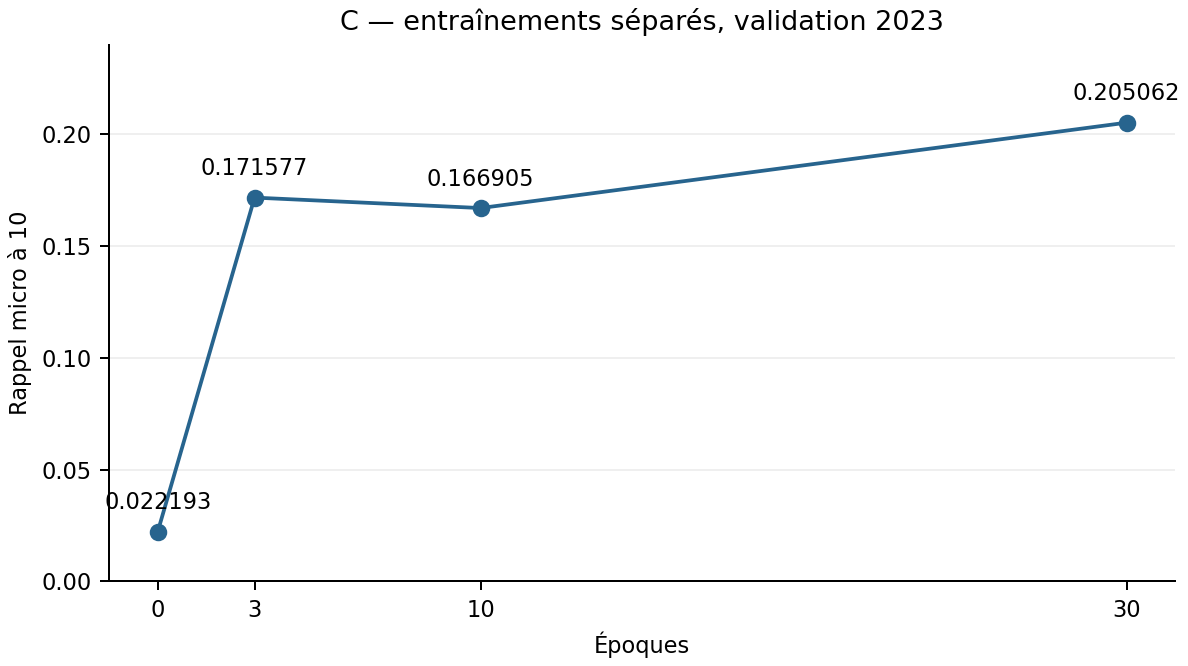
\includegraphics[width=\linewidth]{figures/maude_duration_RC2_fr.png}
\caption{C : rappel micro@10 en validation selon la durée d'entraînement. Le fit à zéro époque n'a aucune perte d'entraînement observée.}
\label{fig:maude-duration-rc2}
\end{figure}

Après le choix, la durée sélectionnée a été ajustée séparément avant 2024 et 2025, avec historique roulant entre les trimestres de test. Au test 2024, le rappel micro@10 est $1\,206/6\,003=0,200899550225$ ; en 2025, $1\,569/7\,171=0,218797936132$. En cumulant les liens retrouvés et les liens positifs des deux années, le rappel atteint $2\,775/13\,174=0,210642173979$, pour 6\,370 produit--trimestres positifs et 2\,975\,156 paires candidates. Ce rappel regroupé n'est pas la moyenne arithmétique des deux rappels annuels.

Le test historique du benchmark donnait 0,172840443297 au GraphSAGE à trois époques et 0,192044936997 à la fréquence des voisins. Ces valeurs historiques restent inchangées. Le résultat C à 30 époques n'est pas un contraste direct entre trois et trente époques sur le test : les tests C ne comprenaient pas un nouveau fit à trois époques. Il s'agit d'une comparaison descriptive entre l'exploration RC2 et les valeurs conservées, sans nouvel intervalle de confiance, bootstrap, sélection sur test ou revendication de supériorité statistique.

\subsection{D1 : comparaison à agrégation moyenne et variante sans voisinage}

D1 compare le modèle \emph{mean} de C à 30 époques, réutilisé sans nouvel ajustement, à un seul nouveau modèle \emph{none} à 30 époques. Le choix commun de durée provient de C et du protocole D1 fixé ; aucune grille ni aucun ajustement de durée n'a été mené dans D1. Les mêmes périodes et règles d'évaluation sont utilisées pour les deux variantes : identifiants de candidats, étiquettes, soutiens, négatifs hachés et conventions de classement concordent. Les deux modèles conservent des vecteurs d'identité de nœuds entraînables. Le modèle \emph{none} calcule $h=\tanh(W_{\mathrm{self}}x)$ à partir du seul vecteur propre du nœud ; il n'agrège pas les voisins et n'est pas un GNN.

La variante \emph{mean} a 128 scalaires de transformations partagées actives, contre 64 pour \emph{none} ; le nombre de scalaires des vecteurs de nœuds est le même dans chaque paire de fits. La variante \emph{none} a donc 64 paramètres actifs de moins dans les trois phases. Le contraste modifie simultanément l'agrégation et le nombre de paramètres des transformations ; il n'isole pas un effet causal de l'agrégation à capacité égale.

Le choix D1 a été verrouillé à 20:53:30.842192 UTC à partir de la validation, avant les premiers tests propres à D1. Cependant, les résultats de test du modèle \emph{mean} issus de C étaient déjà disponibles au moment de ce verrou et les périodes de test avaient déjà été consultées antérieurement. L'ordre du verrou D1 et de ses tests ne transforme donc pas l'analyse en confirmation indépendante.

\begin{table}[!htbp]\centering\scriptsize\setlength{\tabcolsep}{2.5pt}
\caption{D1 : rappel micro@10 sur les cohortes avec au moins un lien positif, au soutien historique $\geq1$. Mean30 est conservé de C ; none30 est nouvellement ajusté dans D1. Les liens retrouvés sont indiqués entre parenthèses. Aucun intervalle n'est associé au contraste.}
\label{tab:aggregation-rc2}
\begin{tabularx}{\linewidth}{@{}XrXXr@{}}
\toprule
Cohorte & Liens positifs & Mean30 R@10 (retrouvés) & None30 R@10 (retrouvés) & Mean $-$ none\\
\midrule
Validation 2023 & 7\,705 & 0,205061648 (1\,580) & 0,031148605 (240) & $+0,173913043$\\
Test 2024 & 6\,003 & 0,200899550 (1\,206) & 0,036481759 (219) & $+0,164417791$\\
Test 2025 & 7\,171 & 0,218797936 (1\,569) & 0,034862641 (250) & $+0,183935295$\\
Test groupé 2024--2025 & 13\,174 & 0,210642174 (2\,775) & 0,035600425 (469) & $+0,175041749$\\
\bottomrule
\end{tabularx}
\end{table}

Sur le test regroupé, mean30 obtient $2\,775/13\,174=0,210642173979$ et none30 $469/13\,174=0,035600425080$ ; l'écart descriptif signé mean30--none30 est $+0,175041748899$. Aucun intervalle de confiance ni test statistique n'est associé à cet écart. La figure indique aussi les contrastes annuels et les pertes enregistrées.

\begin{figure}[!htbp]\centering
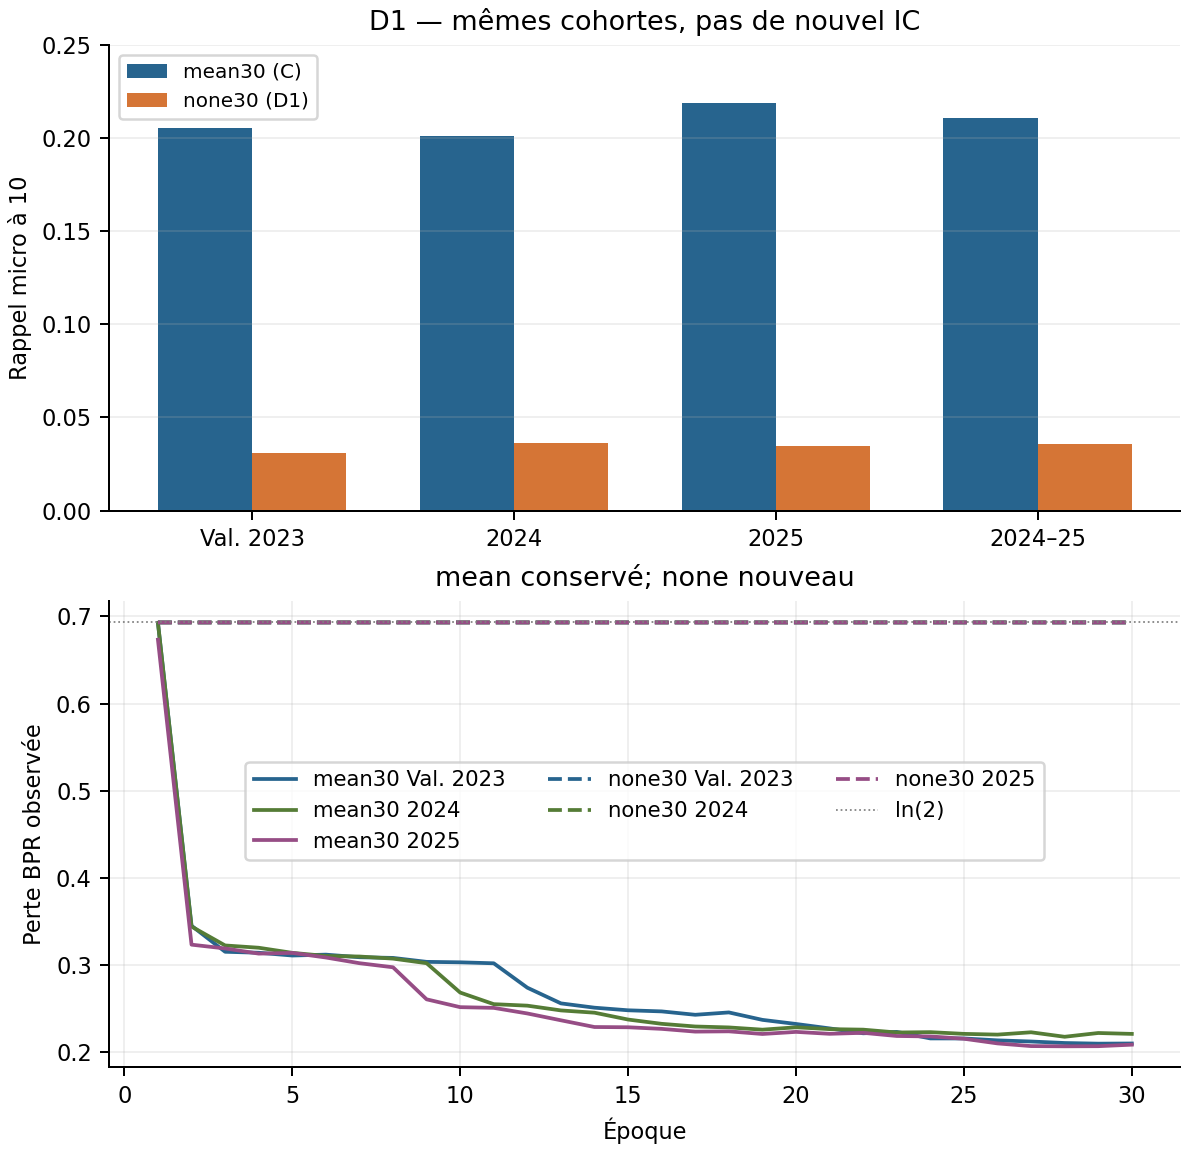
\includegraphics[width=\linewidth]{figures/maude_aggregation_RC2_fr.png}
\caption{D1 : rappels micro@10 dans le panneau supérieur ; pertes observées dans le panneau inférieur. Mean30 est réutilisé de C ; seuls les fits none30 sont nouveaux dans D1. Le rappel regroupé cumule les deux années de test et ne représente pas une cohorte distincte supplémentaire.}
\label{fig:maude-aggregation-rc2}
\end{figure}

Les trois fits none30 comportent 90 époques observées, 6\,756\,720 pas et aucun positif sauté. La perte de données exportée, moyenne de $\operatorname{softplus}(-\text{marge})$ avant mise à jour et hors régularisation, reste proche de $\ln(2)$ sans baisse observée (environ 0,693132--0,693145 à la première époque et 0,693147 à la trentième). C'est la description des journaux obtenus sous ces paramètres ; elle n'identifie pas un mécanisme de performance ni une cause d'échec d'optimisation.

\subsection{Audits, coûts et portée des vérifications}

Les audits C et D1 portent sur les nouveaux fits et ne remplacent pas la reconstruction historique B1/B2 de S10. L'audit C reconstruit les scores à partir de six checkpoints bruts et vérifie 9\,449\,508 prédictions, 24 trimestres-fit et 20\,302 listes candidates ; aucun écart n'est détecté, avec une tolérance absolue de $10^{-12}$ pour les flottants. Le rapport est conservé sous \src{verification/post_rc1/C_numeric_audit.json}, avec le manifeste \src{data/post_rc1/C_manifest.json}. Les reconstructions B1/B2 antérieures reconstituaient entrées d'entraînement et inventaires de nœuds, sans inspection des checkpoints historiques.

L'audit D1 reconstruit les scores none30 depuis trois checkpoints bruts et les apparie aux sorties mean30 conservées de C. Il vérifie 4\,593\,744 nouveaux scores, 9\,853 listes candidates par variante, 12 trimestres et 51\,260\,776 contrôles numériques ; aucun écart n'est détecté à la tolérance absolue $10^{-12}$. Le nombre de 9\,187\,488 identifiants candidats est la somme des deux exports, soit 4\,593\,744 paires de chaque côté. L'audit D1 a duré 58,547 s. Ses mesures mémoire finales divergent : $118\,292\,480$ octets pour \texttt{VmHWM} et \texttt{VmRSS}, contre $571\,580\,416$ octets pour \texttt{ru\_maxrss}. Faute de mesures au démarrage, il n'est pas possible de certifier que l'audit entier est resté sous 512 Mio ni d'attribuer avec certitude la divergence au processus ou au lanceur. Un probe indépendant de télémétrie montre qu'une portée différente après \texttt{exec} peut expliquer la divergence, sans établir l'origine exacte de cette mesure d'audit. Les deux valeurs restent consignées dans \src{data/post_rc1/post_rc1_metrics.json}.

Pour les phases d'entraînement, les limites étaient de 900 s, 512 Mio de RSS agrégée et 512 Mio de sorties par phase, avec un seul travailleur et un environnement monothread ; chaque phase C et D1 rapportée s'est achevée sous ces plafonds, sans nouvelle tentative. C a totalisé 1\,167,908 s entre ses phases (pic RSS agrégé maximal 249\,405\,440 octets) ; ce cumul de plusieurs phases n'était pas soumis à un plafond global de 900 s. D1 a totalisé 416,144 s (pic RSS agrégé maximal 303\,284\,224 octets). Les mesures mean30 sont celles de C et sont réutilisées ; elles ne constituent pas de nouveaux coûts d'ajustement dans D1. Ces coûts ne démontrent pas une égalité des budgets CPU entre variantes ou entre exécutions.

Ces vérifications établissent la cohérence numérique des sorties RC2 avec les instantanés préparés, checkpoints et journaux audités. Elles ne vérifient pas une disponibilité publique historique de chaque champ, ne corrigent pas l'exposition préalable aux périodes, ne fournissent ni confirmation indépendante ni bénéfice clinique et ne justifient aucune inférence causale ou générale sur les graphes.


\section{Éléments ouverts et préparation éditoriale}
\label{supp:open}
RC2 intègre les explorations MAUDE C/D1 de S11 tout en conservant les tableaux historiques. L'avis R6 et la réponse associée restent des pièces historiques : ils ne constituent ni une revue ni une approbation de RC2. Les vérifications techniques du paquet sont consignées dans \src{verification/rc2}; elles ne remplacent pas l'approbation scientifique et bibliographique des auteurs. Le manuscrit n'est ni soumis ni accepté.

La référence RelBench v2 a été corrigée en \emph{3rd DATA-FM Workshop at ICLR 2026}, conformément au lieu imprimé sur la première page de l'article, et non en conférence principale\cite{gu2026relbench}. R3 ajoute une référence précise au contrôle synthétique et harmonise les notes de provenance; aucune nouvelle recherche exhaustive de littérature n'est revendiquée.

La revue cible, ses exigences de longueur, de langue, d'anonymisation et de présentation restent à fixer. Le nom FAIA hérité désigne une collection d'ouvrages et d'actes, non un choix de revue. Les entrées \src{submission_ios_fr.tex} et \src{submission_ios_en.tex} sont destinées à la classe IOS ; elles ne sont pas compilées ou validées ici pour un support final. Les PDF livrés utilisent une maquette de lecture.

Enfin, noms, affiliations, correspondant, contributions, financements, conflits d'intérêts, position éthique, conditions d'utilisation des données et déclaration d'assistance par IA doivent être approuvés par les auteurs. Ne pas remplacer les champs absents par « aucun » ou par une dispense supposée. Les éléments de la réponse aux évaluateurs sont des propositions de réponse documentées, non une attestation signée ni une soumission effectuée.

\bibliographystyle{unsrtnat}
\bibliography{references}
\end{document}
